\documentclass[11pt]{article}

\usepackage{amsmath, amssymb, amsthm, geometry}
\usepackage{tikz-cd}
\usepackage{booktabs}
\usepackage{hyperref}
\geometry{margin=1in}

\title{Kochen--Specker Contextuality as Central Extension:\\
The Peres--Mermin Square and the Pauli Group\\
{\large (Paper III: The Kernel and Group Cohomology)}}


\author{Zhou-Li Chen \\ co-nlang Research}
\date{May 2026}

\newtheorem{theorem}{Theorem}[section]
\newtheorem{proposition}[theorem]{Proposition}
\newtheorem{lemma}[theorem]{Lemma}
\newtheorem{corollary}[theorem]{Corollary}
\newtheorem{definition}[theorem]{Definition}
\newtheorem{remark}[theorem]{Remark}
\newtheorem{conjecture}[theorem]{Conjecture}

\begin{document}

\maketitle

\begin{abstract}
This paper completes a three-paper programme establishing the cohomological
structure of quantum contextuality. Papers I and II constructed the affine
geometric phase map
\[
  R_*: H^1(\mathcal{C}^{\mathrm{BS}}(A),\, \underline{U(1)})
  \longrightarrow \check{H}^1(M,\, U(1))
\]
and showed its image captures the geometrically visible (line bundle) shadow
of quantum phases. This paper addresses the missing piece:
\textbf{what the kernel $\ker(R_*)$ should capture}, via a \emph{discrete model} of
contextual obstructions invisible to line bundles.

We show that the Peres--Mermin square exhibits a central extension
obstruction: the Hermitian Pauli group $\mathcal{P}_2^H$ is a non-split central
extension $1 \to \{\pm I\} \to \mathcal{P}_2^H \to \bar{\mathcal{P}}_2 \to 1$
whose class $[f]$ generates a $\mathbb{Z}/2$ summand corresponding directly to the
symplectic commutator pairing, and evaluates on the Kochen--Specker 2-cycle to $-1$.
This non-trivial evaluation witnesses the Kochen--Specker contradiction via group cohomology.

\textbf{The complete picture.} The three papers together establish a
conjectural short exact sequence:
\[
  0 \longrightarrow \underbrace{\ker(R_*)}_{\text{contextual (modeled in this paper)}}
  \longrightarrow H^1(\mathcal{C}^{\mathrm{BS}}, \underline{U(1)})
  \xrightarrow{\;R_*\;} \underbrace{\check{H}^1(M, U(1))}_{\text{geometric (Papers I--II)}}
\]
Paper~I defined $R_*$; Paper~II identified its image with Riemann surface
periods; this paper computes a discrete model of the kernel via central extension.
\end{abstract}

%------------------------------------------------------------------
\section{Introduction}
%------------------------------------------------------------------

The quest to unify the algebraic and geometric foundations of quantum mechanics has recently centered on two distinct cohomological frameworks. On one hand, \emph{Bohrification} reformulates quantum theory as a sheaf of commutative C*-subalgebras over a poset of contexts \cite{Lan16}. On the other, \emph{Geometric Quantization} encodes quantum structure via line bundles and symplectic geometry on classical phase spaces \cite{BW97}.

In the first two papers of this programme \cite{PaperI, PaperII}, we established a computable bridge between these perspectives by defining the \emph{affine geometric phase map} $R_*$. We proved that the image of this map, $\mathrm{im}(R_*)$, captures the ``geometric shadow'' of quantum phases---those components detectable as holonomies of prequantum line bundles and periods of Riemann surfaces. However, a fundamental question remained: \textbf{what lies in the kernel $\ker(R_*)$?}

This kernel represents the contextual obstructions that possess no line-bundle shadow---the purely non-abelian residue of quantum logic that eludes classical geometric description. This paper addresses this missing piece by shifting the investigation from continuous manifolds to a discrete algebraic setting.

\subsection{The discrete model: A logical prism}

To compute $\ker(R_*)$, we employ a faithful discretization where the continuous Weyl--Heisenberg symmetry of Papers I--II is replaced by the Hermitian Pauli group $\mathcal{P}_2^H$ acting on the $M_4(\mathbb{C})$ observable algebra. In this simplified environment, geometric complications recede, allowing the central extension structure to emerge as the primary witness of contextuality.

Using the Peres--Mermin (PM) square \cite{Peres90, Mermin90} as our discrete testbed, we show that Kochen--Specker contextuality is not merely a logical contradiction, but a failure of algebraic lifting. This lifting obstruction is rigorously encoded in the group cohomology $H^2(\bar{\mathcal{P}}_2, \mathbb{Z}/2)$, providing a bridge between the sheaf-theoretic obstructions of Bohrification and the central extension physics of projective representations.

The central thesis of our programme, now fully articulated, is the following cohomological decomposition:

\begin{quote}
\textbf{The Synthesis Conjecture.} The total phase cohomology of a quantum system fits into a conjectural short exact sequence:
\[
  0 \longrightarrow \underbrace{\ker(R_*)}_{\text{contextual (modeled in this paper)}}
  \longrightarrow H^1(\mathcal{C}^{\mathrm{BS}}, \underline{U(1)})
  \xrightarrow{\;R_*\;} \underbrace{\check{H}^1(M, U(1))}_{\text{geometric (Papers I--II)}}
\]
This paper identifies $\ker(R_*)$ with the central extension class of the symmetry group, completing the three-paper arc from map definition (Paper I) and image identification (Paper II) to kernel evaluation (Paper III).
\end{quote}

\subsection{Structure of the paper}

The remainder of this paper is structured as follows. In Section~\ref{sec:prelim}, we review the theory of central extensions and the Hermitian Pauli group. Section~\ref{sec:PM} defines the Peres--Mermin square and its intersection geometry on the $K_{3,3}$ nerve. In Section~\ref{sec:constraint}, we formalize the lifting problem and introduce the 4-cycle holonomy as a geometric interpretation. Section~\ref{sec:central} presents our main results, constructing the Kochen--Specker 2-cycle and evaluating the central extension class. We conclude in Section~\ref{sec:synthesis} by synthesizing the three-paper programme and outlining directions for future work in field theory and Seiberg--Witten geometry.

\subsection{Relation to existing literature}

Abramsky--Brandenburger \cite{AB11} treat KS contextuality as the
obstruction to a global section of a \emph{presheaf of measurement
outcomes}, encoded in sheaf cohomology. Our construction is categorically
distinct:

\begin{center}
\renewcommand{\arraystretch}{1.4}
\begin{tabular}{lll}
\toprule
& Abramsky--Brandenburger & \textbf{This paper} \\
\midrule
Presheaf & outcomes (values) & operator algebras (Bohrification) \\
Cohomology & sheaf $H^1$ (empirical model) & \textbf{group $H^2$} (central extension) \\
Mechanism & global section obstruction & \textbf{lifting obstruction} \\
\bottomrule
\end{tabular}
\end{center}

\textbf{Note:} A--B compute $H^1$ of the presheaf of empirical models (measurement outcomes);
this paper computes $H^2$ of the Pauli group (operator algebra symmetry).
These measure different obstructions.

\textbf{Key difference:} A--B uses the presheaf of \emph{measurement outcomes}.
We use Bohrification (presheaf of \emph{algebras}) and identify the KS
obstruction with the group cohomology class $[f] \in H^2(\bar{\mathcal{P}}_2, \mathbb{Z}/2)$
that measures the failure to lift the PM observables consistently to $\mathcal{P}_2^H$.

%------------------------------------------------------------------
\section{Mathematical Preliminaries: Central Extensions}
\label{sec:prelim}
%------------------------------------------------------------------

\subsection{Group Extensions and Cohomology}

Let $G$ be a group and $A$ an abelian group. A \emph{central extension}
of $G$ by $A$ is a short exact sequence:
\[
  1 \longrightarrow A \longrightarrow \tilde{G}
  \longrightarrow G \longrightarrow 1
\]
where $A$ lies in the centre of $\tilde{G}$. The set of equivalence
classes of such extensions is classified by the second cohomology
group $H^2(G, A)$.

Explicitly, a 2-cocycle $\alpha \in Z^2(G, A)$ is a map
$\alpha: G \times G \to A$ satisfying:
\begin{equation}
\label{eq:cocycle}
  \alpha(g, h) \cdot \alpha(gh, k)
  = \alpha(g, hk) \cdot \alpha(h, k)
  \quad \forall\, g, h, k \in G.
\end{equation}
Given such a cocycle, the extension $\tilde{G}$ is constructed as the
set $G \times A$ with multiplication:
\[
  (g, a) \cdot (h, b) = (gh, \alpha(g, h) \cdot ab).
\]

\subsection{The Hermitian Pauli Group as Central Extension}
\label{sec:pauli-ext}

The full two-qubit Pauli group is
\[
  \mathcal{P}_2 = \{\pm I, \pm iI\} \cdot \{I,X,Y,Z\}^{\otimes 2},
  \quad |\mathcal{P}_2| = 64,
\]
with centre $Z(\mathcal{P}_2) = \{\pm I, \pm iI\} \cong \mathbb{Z}/4$.
For the central extension construction, we restrict to the
\emph{Hermitian Pauli group}:
\[
  \mathcal{P}_2^H := \{\pm P : P \in \{I,X,Y,Z\}^{\otimes 2}\},
  \quad |\mathcal{P}_2^H| = 32,
\]
consisting of Hermitian operators only (no explicit $i$ factors).
This is the natural subgroup for quantum observables since physical
measurements correspond to Hermitian operators.

The centre of $\mathcal{P}_2^H$ is $Z(\mathcal{P}_2^H) = \{\pm I\} \cong \mathbb{Z}/2$,
and the quotient
\[
  \bar{\mathcal{P}}_2 := \mathcal{P}_2^H / Z(\mathcal{P}_2^H)
  \cong (\mathbb{Z}/2)^4
\]
is a 4-dimensional $\mathbb{F}_2$-vector space with basis
$\bar{X}_1, \bar{Z}_1, \bar{X}_2, \bar{Z}_2$.

\begin{proposition}[Hermitian Pauli group extension]
\label{prop:pauli-ext}
The Hermitian Pauli group $\mathcal{P}_2^H$ fits into a central extension:
\begin{equation}
\label{eq:pauli-ext}
  1 \longrightarrow \{\pm I\} \longrightarrow \mathcal{P}_2^H
  \longrightarrow \bar{\mathcal{P}}_2 \longrightarrow 1.
\end{equation}
The extension class $[f] \in H^2(\bar{\mathcal{P}}_2, \mathbb{Z}/2)$
is generated by the \emph{factor set} (section cocycle) defined as follows.
Choose a section $s: \bar{\mathcal{P}}_2 \to \mathcal{P}_2^H$ (a choice of
lift for each coset). The factor set $f: \bar{\mathcal{P}}_2 \times \bar{\mathcal{P}}_2 \to \{\pm 1\}$ is:
\begin{equation}
\label{eq:factor-set}
  s(\bar{P}) \cdot s(\bar{Q}) = f(\bar{P}, \bar{Q}) \cdot s(\bar{P} + \bar{Q}),
\end{equation}
where $+$ denotes addition in $\bar{\mathcal{P}}_2 = (\mathbb{Z}/2)^4$.
Equivalently, $f(\bar{P}, \bar{Q}) = s(\bar{P})s(\bar{Q})s(\bar{P}+\bar{Q})^{-1}$.
\end{proposition}

\begin{proof}
The factor set satisfies the 2-cocycle identity \eqref{eq:cocycle}
by associativity of $\mathcal{P}_2^H$: comparing
$s(\bar{P})s(\bar{Q})s(\bar{R})$ computed two ways yields exactly
\eqref{eq:cocycle}.\linebreak
Changing the section $s \mapsto s'$ by $s'(\bar{P}) = \eta(\bar{P})s(\bar{P})$
(for $\eta: \bar{\mathcal{P}}_2 \to \{\pm 1\}$) changes $f$ by a coboundary:
\[
\begin{split}
f'(\bar{P},\bar{Q}) &= f(\bar{P},\bar{Q}) \\
&\quad \cdot \eta(\bar{P})\eta(\bar{Q})\eta(\bar{P}+\bar{Q})^{-1}.
\end{split}
\]
Thus $[f]$ is well-defined in $H^2$.
\end{proof}

\begin{remark}[Physical subgroup and the symplectic pairing]
The full Schur multiplier with $\mathbb{Z}/2$ coefficients is
$H^2(\bar{\mathcal{P}}_2, \mathbb{Z}/2) \cong (\mathbb{Z}/2)^{10}$~
\cite{Kar87}.
This decomposes into two summands:
$\wedge^2(\bar{\mathcal{P}}_2) \cong (\mathbb{Z}/2)^6$ (from antisymmetric bilinear forms)
and an $\text{Ext}$ term $\mathrm{Hom}(\bar{\mathcal{P}}_2, \mathbb{Z}/2) \cong (\mathbb{Z}/2)^4$.
The Pauli group extension represents a specific physical subgroup:
the central extension class $[f]$ from Proposition~\ref{prop:pauli-ext}
generates a $\mathbb{Z}/2$ summand corresponding directly to the
\emph{symplectic commutator pairing} in
$\wedge^2((\mathbb{Z}/2)^4) \subseteq H^2$.
This is the subgroup relevant to the Kochen--Specker obstruction,
as its antisymmetrization
$\alpha(\bar{P}, \bar{Q}) = f(\bar{P}, \bar{Q})f(\bar{Q}, \bar{P})^{-1} \in \{\pm 1\}$
explicitly captures the commutation relations $P Q P^{-1} Q^{-1} = \alpha(\bar{P}, \bar{Q}) \cdot I$.

With $U(1)$ coefficients, the full cohomology group is $H^2(\bar{\mathcal{P}}_2, U(1)) \cong (\mathbb{Z}/2)^{10}$. The symplectic commutator pairing forms an antisymmetric summand $\wedge^2(\bar{\mathcal{P}}_2) \cong (\mathbb{Z}/2)^6 \subseteq (\mathbb{Z}/2)^{10}$, and the class $[f]$ maps non-trivially into this summand under the change-of-coefficients map $H^2(-, \mathbb{Z}/2) \to H^2(-, U(1))$ because the commutator phase $[P,Q] \in \{\pm 1\}$ is non-trivial.
\end{remark}

\begin{definition}[PM generation of the Pauli group]
\label{def:pm-subgroup}
The nine PM observables $O_{ij}$ actually generate the entire group $\bar{\mathcal{P}}_2$.
Specifically, the four observables $\bar{O}_{11}, \bar{O}_{12}, \bar{O}_{21}, \bar{O}_{22}$
correspond to the independent basis vectors $\bar{z}_2, \bar{x}_1, \bar{z}_1, \bar{x}_2$. Thus:
\[
  \langle \bar{O}_{ij} : i,j \in \{1,2,3\} \rangle = \bar{\mathcal{P}}_2 \cong (\mathbb{Z}/2)^4.
\]
\end{definition}

\begin{remark}[The canonical section]
\label{rem:restriction}
Because the PM observables generate all of $\bar{\mathcal{P}}_2$, defining a
section $s(\bar{O}_{ij}) = O_{ij}$ on the generators extends to a full section
$s: \bar{\mathcal{P}}_2 \to \mathcal{P}_2^H$. Consequently, the factor set $f$
evaluated on the PM square is the full factor set $f \in Z^2(\bar{\mathcal{P}}_2, \mathbb{Z}/2)$,
and no restriction to a proper subgroup is necessary.
\end{remark}

\subsection{Lifting Problem and Global Obstruction}
\label{sec:lifting}

Given a central extension \eqref{eq:pauli-ext}, a \emph{lifting} of
$\bar{g} \in \bar{\mathcal{P}}_2$ is a choice of $g \in \mathcal{P}_2^H$
with $\pi(g) = \bar{g}$. Lifts are unique up to multiplication by
$\{\pm I\}$.

For a subset $S \subseteq \bar{\mathcal{P}}_2$, a \emph{section} is a
choice of lift $s(\bar{g}) \in \mathcal{P}_2^H$ for each $\bar{g} \in S$.
If $\bar{g}_1 \cdots \bar{g}_k = 0$ in $\bar{\mathcal{P}}_2$ (additive
notation), the corresponding product of lifts satisfies:
\begin{equation}
\label{eq:constraint-sign}
  s(\bar{g}_1) \cdots s(\bar{g}_k)
  = \prod_{i=1}^{k-1} f\bigl(\bar{g}_1 + \cdots + \bar{g}_i, \bar{g}_{i+1}\bigr)
  \cdot I \in \{\pm I\}.
\end{equation}
This product is the \emph{constraint sign} for the relation
$\bar{g}_1 + \cdots + \bar{g}_k = 0$.

\begin{definition}[Global lifting obstruction]
\label{def:global-obs}
Let $\{\bar{g}_1, \ldots, \bar{g}_m\} \subseteq \bar{\mathcal{P}}_2$ be a
collection with specified relations. The \emph{global lifting
obstruction} is the map:
\[
  \text{Obs}: \{\text{sections}\} \longrightarrow \{\pm 1\},
  \quad s \mapsto \prod_{\text{relations}} \epsilon_c
\]
where $\epsilon_c$ is the constraint sign \eqref{eq:constraint-sign}
for relation $c$. If $\text{Obs}(s) = -1$ for all sections $s$, the
lifting problem has no solution.
\end{definition}

\begin{remark}
The global obstruction is independent of the choice of section $s$
because changing $s(\bar{g}) \mapsto -s(\bar{g})$ flips the signs of all
relations containing $\bar{g}$. If $\bar{g}$ appears in an even number
of relations (as in the PM square), the total product is unchanged.
\end{remark}

\subsection{Bar Resolution and Constraint Chains}
\label{sec:bar}

For computations, we use the bar resolution. For $G = \bar{\mathcal{P}}_2$:
\begin{itemize}
\item $C_n(G)$: free abelian group on $n$-tuples $[g_1|\cdots|g_n]$,
      $g_i \in G \setminus \{0\}$;
\item Boundary: $\partial_n[g_1|\cdots|g_n] = [g_2|\cdots|g_n] +
      \sum_{i=1}^{n-1} (-1)^i[\cdots|g_i+g_{i+1}|\cdots] + (-1)^n[g_1|\cdots|g_{n-1}]$.
\end{itemize}

\begin{definition}[Constraint 2-chain]
\label{def:constraint-chain}
For $\bar{a}, \bar{b}, \bar{c} \in G$ with $\bar{a} + \bar{b} + \bar{c} = 0$,
the \emph{constraint 2-chain} is:
\begin{equation}
\label{eq:constraint-2chain}
  d(\bar{a}, \bar{b}, \bar{c}) := [\bar{a}|\bar{b}] + [\bar{a}+\bar{b}|\bar{c}]
  \in C_2(G).
\end{equation}
\end{definition}

The boundary of a constraint 2-chain in the augmented complex ($[0] = 0$) is:
\begin{equation}
\label{eq:constraint-boundary}
  \partial_2 \, d(\bar{a}, \bar{b}, \bar{c}) = [\bar{a}] + [\bar{b}] + [\bar{c}].
\end{equation}

For a 2-cocycle $f \in Z^2(G, \mathbb{Z}/2)$, evaluation on a
2-chain $c = \sum_i n_i [g_i|h_i]$ is:
\begin{equation}
\label{eq:cocycle-eval}
  \langle f, c \rangle := \prod_i f(g_i, h_i)^{n_i} \in \{\pm 1\}.
\end{equation}

\begin{proposition}[Constraint evaluation]
\label{prop:constraint-eval}
Let $\bar{a} + \bar{b} + \bar{c} = 0$ in $G$. For any section $s$, the scalar evaluation of the 2-cocycle on the constraint chain exactly matches the operator constraint sign:
\[
  \langle f, d(\bar{a}, \bar{b}, \bar{c}) \rangle \cdot I
  = s(\bar{a}) s(\bar{b}) s(\bar{c})
  = \epsilon_c \cdot I.
\]
Thus, identifying the scalar $\pm 1$ with the central operator $\pm I$, we rigorously have $\langle f, d(\bar{a}, \bar{b}, \bar{c}) \rangle = \epsilon_c$.
\end{proposition}

\begin{proof}
By Eq.~\eqref{eq:constraint-sign} with $k=3$, the operator product is $s(\bar{a})s(\bar{b})s(\bar{c}) = f(\bar{a}, \bar{b}) f(\bar{a}+\bar{b}, \bar{c}) \cdot I$.
By definition of the cocycle evaluation \eqref{eq:cocycle-eval} on the constraint 2-chain $d(\bar{a},\bar{b},\bar{c}) = [\bar{a}|\bar{b}] + [\bar{a}+\bar{b}|\bar{c}]$, the scalar coefficient is exactly $\langle f, d(\bar{a}, \bar{b}, \bar{c}) \rangle = f(\bar{a}, \bar{b}) f(\bar{a}+\bar{b}, \bar{c})$.
Since the operator product defines the constraint sign $\epsilon_c \cdot I$, the scalar identity $\langle f, d(\bar{a}, \bar{b}, \bar{c}) \rangle = \epsilon_c$ strictly follows.
\end{proof}

%------------------------------------------------------------------
\section{Geometric Interpretation: Parallel Transport}
\label{sec:transport}
%------------------------------------------------------------------

\textbf{Motivation: from continuous to discrete.}
In Papers~I and II, ``parallel transport'' refers to the connection on a
flat line bundle over a continuous symplectic manifold $M$. Here we define
its discrete analogue: while the PM square is finite-dimensional, its MASA
poset forms a $K_{3,3}$ nerve. The ``parallel transport'' between contexts
is the unitary operator that switches between eigenbases of commuting
observables. This bridges the continuous geometric picture (line bundles)
to the discrete algebraic picture (central extensions).

This section provides a geometric interpretation of the algebraic
constraint signs. The central extension obstruction can be understood
as the holonomy of a ``parallel transport'' between contexts.

Let $C_i, C_j \in \mathcal{C}(A)$ be MASAs with intersection
$C_{ij} := C_i \cap C_j \not\cong \mathbb{C}\cdot I$.
There exists a unital $*$-isomorphism
$\Phi_{ij}: C_i \xrightarrow{\;\sim\;} C_j$ restricting to identity on $C_{ij}$.
Any unitary $U_{ij} \in B(\mathcal{H})$ satisfying
$U_{ij}\, a\, U_{ij}^* = \Phi_{ij}(a)$ for all $a \in C_i$
is called a \emph{parallel transport operator}.

Such $U_{ij}$ is unique up to multiplication by elements of the commutant
$C_{ij}'$. For Pauli-generated intersections $C_{ij} = \{O_{ij}\}''$,
the eigenspace decomposition $\mathcal{H} = \mathcal{H}_{ij}^{(+)} \oplus \mathcal{H}_{ij}^{(-)}$
yields $C_{ij}' \cong M_2(\mathbb{C}) \oplus M_2(\mathbb{C})$.

\begin{definition}[Canonical lift]
\label{def:canonical}
The \emph{canonical} parallel transport $U_{R_i C_j}^{\mathrm{can}}$
is defined by mapping the ordered joint eigenbasis of $R_i$ on each
$\mathcal{H}_{ij}^{(\lambda)}$ to the corresponding ordered eigenbasis
of $C_j$. See Appendix~\ref{app:transport-proof} for the algebraic proof.
\end{definition}

\begin{definition}[Parallel transport and holonomy]
\label{def:holonomy}
Let $U_{ij}$ be any unitary intertwining MASAs $C_i$ and $C_j$, meaning
$U_{ij} M U_{ij}^\dagger = \Phi_{ij}(M)$ for all $M \in C_i$, where
$\Phi_{ij}$ is the canonical algebra isomorphism fixing the shared observable.
For a 4-cycle $R_i \to C_j \to R_k \to C_l \to R_i$ in $K_{3,3}$,
the \emph{holonomy operator} is the product:
\begin{equation}
\label{eq:holonomy}
\sigma_{ijkl} := U_{R_i C_j} \cdot U_{C_j R_k} \cdot U_{R_k C_l} \cdot U_{C_l R_i}
\;\in\; \mathcal{P}_2.
\end{equation}
This operator is related to the composite cycle isomorphism $\Phi_{\mathrm{cyc}}$
on the initial MASA $R_i$ \emph{up to the central extension obstruction}:
conjugation by $\sigma$ gives the identity when $\sigma = -I$ is central,
while $\Phi_{\mathrm{cyc}}$ is an algebra automorphism requiring a specific
Pauli operator ($Z \otimes I$) for its implementation. The discrepancy
between the geometric transport product ($-I$) and the algebraic requirement
($Z \otimes I$) is the holonomy discrepancy.
\end{definition}

The following conjecture shows that the algebraic parallel transport
detects the Kochen--Specker obstruction through the \emph{holonomy discrepancy}:
the geometric transport yields a scalar, while the algebraic implementation
requires a non-central Pauli operator.
The rigorous algebraic argument (Appendix~\ref{app:transport-proof}) relies
directly on the product constraint discrepancies, avoiding any basis-dependent
matrix ambiguities.

\begin{conjecture}[Holonomy Discrepancy]
\label{thm:holonomy-statement}
For the anomalous 4-cycle $R_3 \to C_3 \to R_1 \to C_1 \to R_3$, the KS
constraint discrepancy forces the composite cycle isomorphism $\Phi_{\mathrm{cyc}}$
on $R_3$ to act as:
\[
  \Phi_{\mathrm{cyc}}(O_{31}) = O_{31}, \quad \Phi_{\mathrm{cyc}}(O_{32}) = -O_{32}, \quad \Phi_{\mathrm{cyc}}(O_{33}) = -O_{33}.
\]
This algebra automorphism on $R_3$ can be implemented by conjugation via the Pauli operator $Z \otimes I$.
However, the actual holonomy operator $\sigma \in \mathcal{P}_2^H$ obtained by the product of geometric parallel transports is conjectured to be the central scalar:
\begin{equation}
\label{eq:holonomy-statement}
\sigma_{R_3 C_3 R_1 C_1} = -I.
\end{equation}
The discrepancy between the transport product ($\sigma = -I$) and the required implementing Pauli operator ($Z \otimes I$) is the central extension obstruction, reflecting the constraint sign ratio $\epsilon_{C_3}/\epsilon_{R_3} = -1$.
\end{conjecture}

%------------------------------------------------------------------
\section{The Peres--Mermin Square}
\label{sec:PM}
%------------------------------------------------------------------

\subsection{Observables and contexts}

The PM square consists of nine observables in $M_4(\mathbb{C})$:
\[
\begin{pmatrix}
  O_{11} = I{\otimes}Z & O_{12} = X{\otimes}I & O_{13} = X{\otimes}Z \\[4pt]
  O_{21} = Z{\otimes}I & O_{22} = I{\otimes}X & O_{23} = Z{\otimes}X \\[4pt]
  O_{31} = Z{\otimes}Z & O_{32} = X{\otimes}X & O_{33} = {-Y{\otimes}Y}
\end{pmatrix}
\]
where $X, Y, Z$ are the Pauli matrices.

\textbf{Commutativity.} Within each row $R_k$ and each column $C_k$,
the three observables mutually commute. Hence each row and column
generates a MASA:
\[
  R_k = \{O_{k1}, O_{k2}, O_{k3}\}'',\quad
  C_k = \{O_{1k}, O_{2k}, O_{3k}\}'', \quad k = 1, 2, 3.
\]

\textbf{Product constraints.}
\begin{align}
  &O_{k1} O_{k2} O_{k3} = +I \quad\text{(each row } k\text{)}, \label{eq:row}\\
  &O_{1k} O_{2k} O_{3k} = +I \quad (k=1,2),\quad
   O_{13} O_{23} O_{33} = -I \quad (k=3). \label{eq:col}
\end{align}

The sign discrepancy in~\eqref{eq:col} is the PM contradiction.

\subsection{Intersection structure}

The MASA poset for the PM square has the following intersection
structure: for $i, j \in \{1,2,3\}$,
\[
  R_i \cap C_j = \{O_{ij}\}'', \quad \dim(R_i \cap C_j) = 2
  \;\text{(as vector space over }\mathbb{C}\text{)}.\linebreak
\]
Each intersection is generated by a single Pauli observable,\linebreak giving a $4$-element MASA ($\{I, O_{ij}, P_{ij}^+, P_{ij}^-\}$ where $P_{ij}^\pm$ are rank-2 spectral projections).

\begin{remark}[Poset geometry]
The 6 MASAs $\{R_1, R_2, R_3, C_1, C_2, C_3\}$ with their 9
pairwise intersections $\{R_i \cap C_j\}$ form the combinatorial
structure of the complete bipartite graph $K_{3,3}$, embedded in
$\mathcal{C}(A)$. This is the nerve of the PM covering.
\end{remark}

\begin{figure}[h]
\centering
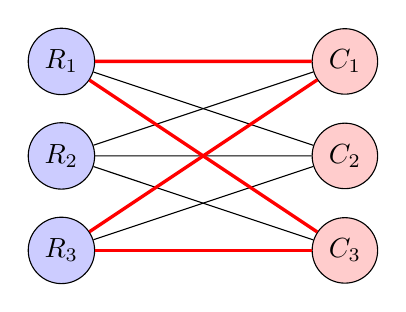
\begin{tikzpicture}[scale=1.2]
% Row nodes (left side)
\node[draw, circle, fill=blue!20] (R1) at (0,2) {$R_1$};
\node[draw, circle, fill=blue!20] (R2) at (0,1) {$R_2$};
\node[draw, circle, fill=blue!20] (R3) at (0,0) {$R_3$};

% Column nodes (right side)
\node[draw, circle, fill=red!20] (C1) at (3,2) {$C_1$};
\node[draw, circle, fill=red!20] (C2) at (3,1) {$C_2$};
\node[draw, circle, fill=red!20] (C3) at (3,0) {$C_3$};

% Edges (topology is clear without labels; the graph structure matters more than edge labels)
\draw (R1) -- (C1);
\draw (R1) -- (C2);
\draw (R1) -- (C3);
\draw (R2) -- (C1);
\draw (R2) -- (C2);
\draw (R2) -- (C3);
\draw (R3) -- (C1);
\draw (R3) -- (C2);
\draw (R3) -- (C3);

% Anomalous 4-cycle highlighted
\draw[very thick, red] (R3) -- (C3);
\draw[very thick, red] (C3) -- (R1);
\draw[very thick, red] (R1) -- (C1);
\draw[very thick, red] (C1) -- (R3);

\end{tikzpicture}
\caption{The $K_{3,3}$ graph of the PM square. Rows (blue) connect to
columns (red). The \textbf{anomalous 4-cycle} $R_3 \to C_3 \to R_1 
\to C_1 \to R_3$ is highlighted (thick red edges).}
\label{fig:k33}
\end{figure}

%------------------------------------------------------------------
\section{Constraint Signs and the Global Lifting Obstruction}
\label{sec:constraint}
%------------------------------------------------------------------

These constraint signs $\epsilon_c$ are precisely the obstructions
encountered when choosing lifts of $\bar{O}_{ij} \in \bar{\mathcal{P}}_2$
to $\mathcal{P}_2^H$; they constitute the concrete realization of the
lifting problem from Section~\ref{sec:lifting} in the PM square.

\subsection{Product constraints in the PM square}

Recall the PM square observables from Section~\ref{sec:PM}:
\[
\begin{pmatrix}
O_{11}=I{\otimes}Z & O_{12}=X{\otimes}I & O_{13}=X{\otimes}Z \\
O_{21}=Z{\otimes}I & O_{22}=I{\otimes}X & O_{23}=Z{\otimes}X \\
O_{31}=Z{\otimes}Z & O_{32}=X{\otimes}X & O_{33}=-Y{\otimes}Y
\end{pmatrix}
\]

Each row $R_k$ and column $C_k$ forms a commutative context. The
\emph{product constraints} are:
\begin{align}
\label{eq:row-constraints}
&O_{k1} O_{k2} O_{k3} = +I \quad\text{(each row $k=1,2,3$)}, \\
\label{eq:col-constraints}
&O_{1k} O_{2k} O_{3k} = +I \quad (k=1,2),\quad
O_{13} O_{23} O_{33} = -I \quad (k=3).
\end{align}

The sign discrepancy in the last column is the PM contradiction.

\subsection{Constraint signs}

\begin{definition}[Constraint sign]
\label{def:constraint-sign}
For a context $c \in \{R_1, R_2, R_3, C_1, C_2, C_3\}$, the
\emph{constraint sign} $\epsilon_c \in \{\pm 1\}$ is defined by:
\begin{equation}
\label{eq:epsilon-c}
\prod_{O_{ij} \in c} O_{ij} = \epsilon_c \cdot I \in \{\pm I\}.
\end{equation}
Explicitly:
\begin{align*}
\epsilon_{R_1} &= +1 &(O_{11} O_{12} O_{13} = +I), &\quad
\epsilon_{R_2} &= +1 &(O_{21} O_{22} O_{23} = +I), &\quad
\epsilon_{R_3} &= +1 &(O_{31} O_{32} O_{33} = +I), \\
\epsilon_{C_1} &= +1 &(O_{11} O_{21} O_{31} = +I), &\quad
\epsilon_{C_2} &= +1 &(O_{12} O_{22} O_{32} = +I), &\quad
\epsilon_{C_3} &= -1 &(O_{13} O_{23} O_{33} = -I).
\end{align*}
\end{definition}

\begin{remark}[Projection to $\bar{\mathcal{P}}_2$]
The operators $\{\pm I\}$ are precisely the kernel of the projection
$\pi: \mathcal{P}_2^H \to \bar{\mathcal{P}}_2$ (the central
subgroup $\{\pm I\} = Z(\mathcal{P}_2^H)$).
In the quotient $\bar{\mathcal{P}}_2$, all constraint signs project
to $0$ (additive notation).
\end{remark}

\subsection{Global lifting obstruction}

The constraint signs encode the \emph{lifting problem} for the central
extension \eqref{eq:pauli-ext}.

\begin{lemma}[Global obstruction]
\label{lem:global-obs}
For any choice of lifts $\tilde{O}_{ij} \in \mathcal{P}_2^H$ of the
nine PM observables $\bar{O}_{ij} \in \bar{\mathcal{P}}_2$ (where each
$\tilde{O}_{ij} = \pm O_{ij}$), let $\tilde{\epsilon}_c \in \{\pm 1\}$ be
the constraint signs computed with these lifts, satisfying
$\prod_{\tilde{O}_{ij} \in c} \tilde{O}_{ij} = \tilde{\epsilon}_c \cdot I$.
Then the product of all six constraint signs satisfies:
\begin{equation}
\label{eq:global-obs}
\prod_{k=1}^3 \tilde{\epsilon}_{R_k} \cdot \prod_{k=1}^3 \tilde{\epsilon}_{C_k}
= -1 \in \{\pm 1\}.
\end{equation}
\end{lemma}

\begin{proof}
Compute the product of all six constraint operators using the constraint sign definition.
The row constraint operators give:
\[
\prod_{k=1}^3 \Bigl(\prod_{\tilde{O}_{ij} \in R_k} \tilde{O}_{ij}\Bigr)
= (+I)(+I)(+I) = +I.
\]
The column constraint operators give:
\[
\prod_{k=1}^3 \Bigl(\prod_{\tilde{O}_{ij} \in C_k} \tilde{O}_{ij}\Bigr)
= (+I)(+I)(-I) = -I.
\]
Thus the product of all six constraint \emph{operators} equals $(+I) \cdot (-I) = -I$.

Translating to signs: since $(+I) = (+1) \cdot I$ and $(-I) = (-1) \cdot I$,
if $\prod_{c} \tilde{O}_{ij} = \tilde{\epsilon}_c \cdot I$,
then the product of all six constraint signs is:
\[
\prod_{k=1}^3 \tilde{\epsilon}_{R_k} \cdot \prod_{k=1}^3 \tilde{\epsilon}_{C_k}
= -1 \in \{\pm 1\}.
\]

For arbitrary lifts $\tilde{O}_{ij} = \pm O_{ij}$, changing the sign of
$\tilde{O}_{ij}$ flips the signs of exactly two constraints (its row and
its column). Thus the product of all six constraint signs changes by $(-1)^{2} = +1$
and remains $-1$ for any choice of lifts.

Since the product equals $-1$, no choice of lifts can make all six constraint signs equal $+1$.
\end{proof}

\begin{corollary}[No consistent lifting]
\label{cor:no-lifting}
There is no choice of lifts $\tilde{O}_{ij} \in \mathcal{P}_2^H$ such that
all six constraint signs equal $+1$ simultaneously.
\end{corollary}

This is the Kochen--Specker theorem expressed as a lifting obstruction.

\subsection{4-Cycle holonomy and local discrepancy}

The holonomy operator $\sigma$ (Definition~\ref{def:holonomy})
measures the \emph{local} discrepancy between constraint signs.
As proven in Appendix~\ref{app:transport-proof}, traversing the anomalous
4-cycle $R_3 \to C_3 \to R_1 \to C_1 \to R_3$ yields an algebra isomorphism
$\Phi_{\mathrm{cyc}}$ that reflects the constraint conflict:
\begin{equation}
\label{eq:holonomy-ratio}
\Phi_{\mathrm{cyc}}(O_{33}) = \left( \frac{\epsilon_{C_3}}{\epsilon_{R_3}} \cdot \frac{\epsilon_{C_1}}{\epsilon_{R_1}} \right) O_{33} = -O_{33}.
\end{equation}
Because $\Phi_{\mathrm{cyc}}$ flips the signs of $O_{32}$ and $O_{33}$ while
fixing $O_{31}$ within the commutative MASA $R_3$, it requires a specific Pauli
operator ($Z \otimes I$) for algebraic implementation. However, the geometric
parallel transport around the cycle is conjectured to yield $\sigma = -I$, a central scalar
(Conjecture~\ref{thm:holonomy-statement}).
The discrepancy between the transport product ($-I$) and the required
implementing operator ($Z \otimes I$) is the holonomy discrepancy. The
Kochen--Specker constraint ratio $\epsilon_{C_3}/\epsilon_{R_3} = -1$ forces
this mismatch, manifesting as the central extension obstruction.

\begin{remark}
The constraint ratio formula \eqref{eq:holonomy-ratio} shows that
$\sigma = -1$ detects the local discrepancy between the $-I$ constraint
sign in column 3 and the $+I$ signs elsewhere. This is a \emph{local
witness} of the global lifting obstruction from Lemma~\ref{lem:global-obs}.
\end{remark}

%------------------------------------------------------------------
\section{Central Extension Evaluation and the Main Theorem}
\label{sec:central}
%------------------------------------------------------------------

\subsection{The Kochen--Specker 2-cycle}

Recall the PM square observables and product constraints from
Section~\ref{sec:PM} (Eqs.~\ref{eq:row}--\ref{eq:col}).
To connect the global lifting obstruction to group cohomology, we must construct a proper closed 2-cycle in the bar complex $C_2(\bar{\mathcal{P}}_2)$. While the contradiction appears locally at the third row and column, a homologically well-defined evaluation requires integrating over the entire PM context structure.

\begin{definition}[Kochen--Specker 2-cycle]
\label{def:ks-cycle}
In the bar complex $C_2(\bar{\mathcal{P}}_2)$, define the \emph{Kochen--Specker 2-cycle} as the alternating sum of the constraint 2-chains for all columns and rows:
\begin{equation}
\label{eq:cks}
c_{\mathrm{KS}} := \sum_{j=1}^3 d(C_j) - \sum_{i=1}^3 d(R_i),
\end{equation}
where $d(C_j) = d(\bar{O}_{1j}, \bar{O}_{2j}, \bar{O}_{3j})$ and $d(R_i) = d(\bar{O}_{i1}, \bar{O}_{i2}, \bar{O}_{i3})$.
\end{definition}

\begin{lemma}[Closed cycle property]
\label{lem:closed}
$c_{\mathrm{KS}}$ is a closed 2-cycle, i.e., $\partial_2 c_{\mathrm{KS}} = 0 \in C_1(\bar{\mathcal{P}}_2)$.
\end{lemma}
\begin{proof}
By Eq.~\eqref{eq:constraint-boundary}, the boundary of each constraint 2-chain is $\partial_2 d(\bar{a}, \bar{b}, \bar{c}) = [\bar{a}] + [\bar{b}] + [\bar{c}]$. Applying this to the Kochen--Specker 2-chain:
\[
\partial_2 c_{\mathrm{KS}} = \sum_{j=1}^3 \bigl( [\bar{O}_{1j}] + [\bar{O}_{2j}] + [\bar{O}_{3j}] \bigr) - \sum_{i=1}^3 \bigl( [\bar{O}_{i1}] + [\bar{O}_{i2}] + [\bar{O}_{i3}] \bigr).
\]
In the bar complex $C_1(\bar{\mathcal{P}}_2)$, this is a formal linear combination of the 1-cells $[\bar{O}_{ij}]$. Because every PM observable $\bar{O}_{ij}$ appears exactly once in the first double sum (iterating over columns) and exactly once in the second double sum (iterating over rows), their coefficients in the difference are exactly $1 - 1 = 0$. Thus, all terms perfectly cancel, yielding $\partial_2 c_{\mathrm{KS}} = 0 \in C_1(\bar{\mathcal{P}}_2)$. Therefore, $c_{\mathrm{KS}}$ is a rigorous 2-cycle in $Z_2(\bar{\mathcal{P}}_2, \mathbb{Z})$.
\end{proof}

Because $c_{\mathrm{KS}}$ is a true 2-cycle, its evaluation against any 2-cocycle $[f] \in H^2(\bar{\mathcal{P}}_2, \mathbb{Z}/2)$ is a rigorously well-defined cohomological invariant, independent of the choice of section $s$.

\textbf{Physical interpretation:} The chain $c_{\mathrm{KS}}$ encodes the difference between all column and row product constraints. The third row and third column intersect at $O_{33} = -Y \otimes Y$, where the row-3 constraint requires $O_{31} O_{32} O_{33} = +I$, while the column-3 constraint requires $O_{13} O_{23} O_{33} = -I$. The Kochen--Specker contradiction---that no assignment of $\pm 1$ values satisfies all six constraints---is precisely the statement that $c_{\mathrm{KS}}$ evaluates non-trivially.

\subsection{Main theorem}

\begin{theorem}[Central extension evaluation]
\label{thm:central}
Let $[f] \in H^2(\bar{\mathcal{P}}_2, \mathbb{Z}/2)$ be the Pauli group central extension class from Proposition~\ref{prop:pauli-ext}. It evaluates on the Kochen--Specker 2-cycle as:
\begin{equation}
\label{eq:main-eval}
\langle f, c_{\mathrm{KS}} \rangle
= \frac{\prod_{j=1}^3 \epsilon_{C_j}}{\prod_{i=1}^3 \epsilon_{R_i}}
= -1 \in \{\pm 1\} \cong \mathbb{Z}/2.
\end{equation}
\end{theorem}

\begin{proof}
By Proposition~\ref{prop:constraint-eval}, for any context $c$, the scalar evaluation is $\langle f, d(c) \rangle = \epsilon_c$.
Since the identity operators cancel, the evaluation on the Kochen--Specker 2-cycle is the ratio of these scalar constraint signs:
\[
\langle f, c_{\mathrm{KS}} \rangle
= \frac{\langle f, d(C_1) \rangle \langle f, d(C_2) \rangle \langle f, d(C_3) \rangle}{\langle f, d(R_1) \rangle \langle f, d(R_2) \rangle \langle f, d(R_3) \rangle}
= \frac{\epsilon_{C_1} \epsilon_{C_2} \epsilon_{C_3}}{\epsilon_{R_1} \epsilon_{R_2} \epsilon_{R_3}}
= \frac{(+1)(+1)(-1)}{(+1)(+1)(+1)} = -1 \in \{\pm 1\}.
\]
\end{proof}

\begin{corollary}[KS contextuality = non-split extension]
\label{cor:ks-central}
The Peres--Mermin square exhibits a non-trivial central extension
obstruction: the factor set $[f]$ generates a $\mathbb{Z}/2$ summand
corresponding directly to the symplectic commutator pairing in
$H^2(\bar{\mathcal{P}}_2, \mathbb{Z}/2) \cong (\mathbb{Z}/2)^{10}$.
Equivalently, the Pauli group extension \eqref{eq:pauli-ext} is
\emph{non-split} when restricted to the PM observable subgroup.
\end{corollary}

\begin{proof}
If the extension were split over the PM observables, there would exist
a section $s$ with all constraint products equal to $+I$. Then
$\langle f, c_{\mathrm{KS}} \rangle = +1$.
Theorem~\ref{thm:central} shows $\langle f, c_{\mathrm{KS}} \rangle = -1$,
so no such splitting exists. The obstruction is precisely the Kochen--Specker
contradiction, encoded cohomologically.
\end{proof}

\subsection{Summary: Three equivalent perspectives}

The KS obstruction admits three equivalent characterizations,
unified by the central extension framework:

\begin{center}
\renewcommand{\arraystretch}{1.4}
\begin{tabular}{lll}
\toprule
\textbf{Perspective} & \textbf{Object} & \textbf{Formula} \\
\midrule
Factor set evaluation & Group cohomology & $\langle f, c_{\mathrm{KS}} \rangle = -1$ \\
Constraint signs & Product constraints & $\epsilon_{C_3}/\epsilon_{R_3} = -1$ \\
4-cycle holonomy & Parallel transport & $\sigma_{R_3 C_3 R_1 C_1} = -1$\textsuperscript{${\dagger}$} \\
\bottomrule
\end{tabular}\\
\vspace{4pt}
\small\textsuperscript{${\dagger}$}Conjectural; see Conjecture~\ref{thm:holonomy-statement}.
\end{center}

The first is the algebraic core: the factor set measures the failure
of the section $s$ to be a homomorphism. The second is the physical
manifestation in the PM square. The third provides a geometric
interpretation via unitary parallel transport (see
Appendix~\ref{app:transport-proof} for the algebraic argument and conjecture).

%------------------------------------------------------------------
\section{Synthesis and Future Directions}
\label{sec:synthesis}
%------------------------------------------------------------------

\subsection{The Three-Paper Decomposition (Conjectural Exact Sequence)}

The three papers together establish a decomposition of contextual
obstructions:

\begin{remark}[Research programme: Synthesis]
\label{conj:synthesis}
Returning to the core sequence introduced in Section~1, we can now formally
articulate the complete decomposition of contextual obstructions:

\textbf{For compact integrable systems:} Papers~I and II construct the map
$R_*$ for algebras arising from Bohr--Sommerfeld quantization of symplectic
manifolds. The conjectured decomposition is:
\[
  0 \;\longrightarrow\; \ker(R_*)
  \;\longrightarrow\; H^1(\mathcal{C}^{\mathrm{BS}}(A),\, \underline{U(1)})
  \;\xrightarrow{\;R_*\;}
  \check{H}^1(M,\, U(1))
\]
where $\mathrm{im}(R_*)$ is the geometric (line bundle) component and
$\ker(R_*)$ is the logical (central extension) component.
The heuristic justification and roadmap for proving exactness are
discussed in Section~\ref{subsec:roadmap} below.

\textbf{For finite-dimensional algebras:} The PM square ($A = M_4(\mathbb{C})$)
is a \emph{faithful discretization} of the continuous framework.
The PM square is the finite $\mathbb{Z}/2$ analogue of the Weyl-Heisenberg group:
Paper~I's continuous BS leaves correspond to the PM square's MASAs,
and the $U(1)$ phase group corresponds to $\{\pm 1\} \cong \mathbb{Z}/2$.
This makes the central extension computation the discrete shadow of
the same cohomological structure. Here:
\begin{itemize}
  \item $\mathcal{C}^{\mathrm{BS}}(A)$ is undefined---the BS construction
        applies to continuous phase spaces, not discrete algebras.
  \item $R_*$ is not directly applicable; the poset $\mathcal{C}(A)$ is
        purely combinatorial.
  \item The KS obstruction is computed by central extension evaluation
        $\langle f, c_{\mathrm{KS}} \rangle = -1$ matching the
        factor set.
\end{itemize}

The PM square computation shows that the \emph{spirit} of the programme
holds: the central extension class $[f]$ is the group-cohomological encoding
of the KS obstruction. The evaluation $\langle f, c_{\mathrm{KS}} \rangle = -1$
serves as the non-trivial \emph{witness} that $[f] \neq 0$, confirming the extension
is non-split. This discrete calculation serves as a faithful algebraic model
for $\ker(R_*)$, rather than a direct continuous computation.
\end{remark}

\begin{center}
\renewcommand{\arraystretch}{1.4}
\begin{tabular}{lp{2.3cm}p{2.7cm}p{3.2cm}}
\toprule
& Paper I & Paper II & Paper III \\
\midrule
Object & map $R_*$ & domain of $R_*$ & $\ker(R_*)$ \\
Tool & Maslov + \v{C}ech & \'etale isomorphism & \textbf{central extension} \\
Result & $[R_*(s_j)] = [\mathcal{P}_\hbar]$ & $\mathrm{Et}(f^*\underline{\mathbb{A}}) \cong \Sigma$ & $\langle f, c_{\mathrm{KS}} \rangle = -1$ \\
Cohomology & $H^1$ & $H^1$ & \textbf{$H^2$ (central ext.)} \\
Physics & Line bundle & Riemann surface & \textbf{Central extension} \\
\bottomrule
\end{tabular}
\end{center}

The central thesis of the programme:

\begin{quote}
\textbf{Bohrification sees the full monodromy of the quantum system.
Geometric quantization sees only its abelian shadow (line bundle, $H^1$).
The non-abelian residue---the Kochen--Specker obstruction---is detected
by central extension evaluation $\langle f, c_{\mathrm{KS}} \rangle = -1$,
corresponding to the non-split extension $1 \to \{\pm I\} \to \mathcal{P}_2^H \to
\bar{\mathcal{P}}_2 \to 1$.}
\end{quote}

\subsection{Discrete Model for the Kernel}

The PM square computation serves as the algebraic anchor for this programme:
the KS obstruction is purely logical, possesses no line bundle shadow,
and is faithfully captured by $\langle f, c_{\mathrm{KS}} \rangle = -1$.

This paper computes the kernel $\ker(R_*)$ via a \emph{faithful discretization}
of the continuous framework from Papers~I--II. The key observation:

\begin{itemize}
  \item \textbf{Continuous (Papers~I--II):} The geometric shadow of quantum
        phases lives in $\check{H}^1(M, U(1))$ (line bundles). The kernel
        consists of contextual obstructions invisible to these geometric
        invariants.

  \item \textbf{Discrete (This paper):} For the PM square, the geometric
        structure degenerates (the base space is discrete). The kernel emerges
        cleanly as the group cohomology $H^2(\bar{\mathcal{P}}_2, \mathbb{Z}/2)$
        classifying central extensions---the non-abelian residue of quantum
        contextuality.
\end{itemize}

The PM square is not a direct instance of the continuous framework, but
a \emph{discrete algebraic model} that isolates and computes the same
kernel structure. The \v{C}ech cohomology of the MASA poset nerve
($\check{H}^2$) vanishes for discrete posets, while the group cohomology
$H^2$ of the symmetry group captures the obstruction.

\subsection{Limitations and Open Questions}

\begin{enumerate}
  \item \textbf{Čech vs.\ group cohomology bridge.} The synthesis between
        sheaf cohomology of the poset nerve and group cohomology of the
        symmetry group requires further development. No direct functorial
        map $H^2_{\text{group}} \to \check{H}^2_{\text{nerve}}$ is provided.

  \item \textbf{Exact sequence conjecture.} The following conjectural
        synthesis remains open for the \emph{continuous} case:
        \[
          0 \longrightarrow \ker(R_*)
          \longrightarrow H^1(\mathcal{C}^{\mathrm{BS}}(A),\, \underline{U(1)})
          \xrightarrow{R_*} \check{H}^1(M,\, U(1))
        \]
        Functoriality of $R_*$ and exactness require a fully developed
        translation between symplectic geometry and topos theory.

  \item \textbf{Canonical lift conventions.} The 4-cycle holonomy
        (Appendix~\ref{app:transport-proof}) depends on basis ordering
        conventions, though the conjectured value $\sigma = -1$ is expected to be independent.
\end{enumerate}

%------------------------------------------------------------------
\subsection{Roadmap to a Rigorous Proof}
\label{subsec:roadmap}
%------------------------------------------------------------------

To elevate this heuristic framework to a strict categorical theorem, the conjectural exact sequence must be grounded in the structural properties of group cohomology. The natural foundation for this is the \emph{Lyndon--Hochschild--Serre (LHS) spectral sequence} associated with the Pauli group central extension.

For the extension $1 \to \{\pm I\} \to \mathcal{P}_2^H \to \bar{\mathcal{P}}_2 \to 1$, the $d_2$ transgression map connects the coefficient group representations to the central extension class:
\[
  d_2: E_2^{0,1} = \mathrm{Hom}(\{\pm I\}, U(1))^{\bar{\mathcal{P}}_2} \longrightarrow E_2^{2,0} = H^2(\bar{\mathcal{P}}_2, U(1)).
\]
The single non-trivial element in $\mathrm{Hom}(\{\pm I\}, U(1))$ is the sign character $\chi_{\mathrm{sign}}$. The standard transgression yields exactly our factor set class: $d_2(\chi_{\mathrm{sign}}) = [f]$.
Our explicit evaluation $\langle f, c_{\mathrm{KS}} \rangle = -1$ serves as the rigorous \emph{witness} that $[f] \neq 0$. Consequently, $[f]$ does not lie in the kernel of the spectral sequence differentials, proving the extension is non-split and the Kochen--Specker obstruction is cohomologically realized.

To fully link this group-cohomological structure back to the Bohrification framework (the exact sequence of Section 7.1), future work must establish the precise functorial relationship between the LHS 5-term exact sequence and the $R_*$ map. This requires constructing natural isomorphisms $\Phi$ and $\Psi$ satisfying the following commutative diagram:

\[
\begin{tikzcd}[row sep=large, column sep=huge]
  H^1(\mathcal{C}^{\mathrm{BS}}(A), \underline{U(1)}) \arrow[r, "R_*"] \arrow[d, dashed, "\Phi"] & \check{H}^1(M, U(1)) \arrow[d, dashed, "\Psi"] \\
  H^1(\mathcal{P}_2^H, U(1)) \arrow[r, "\mathrm{res}"] & H^1(\bar{\mathcal{P}}_2, U(1))
\end{tikzcd}
\]

Here, the bottom row is the exact restriction map from the LHS sequence, mapping the full quantum group representations to the classical (abelian) quotient. The top row is our affine geometric phase map. If the vertical equivalences $\Phi$ and $\Psi$ are constructed, the conjectural decomposition of $R_*$ inherits strict exactness directly from the LHS spectral sequence.

This functorial bridge between topos cohomology and group cohomology stands as the ultimate objective for fully formalizing the geometry of quantum contextuality.

%------------------------------------------------------------------
\subsection{Extensions to Other Systems}
\label{subsec:extensions}
%------------------------------------------------------------------

\begin{enumerate}
  \item \textbf{Larger KS configurations.} The 13-vector Peres configuration
        \cite{Peres90} and the Cabello-Estebaranz-Garcia-Alcaine (CEGA)
        setup \cite{CEGA96} have more complex contextuality. The central extension
        framework should extend, with potentially richer $H^2$ structure.

  \item \textbf{Mermin-Peres magic square game.} The PM square is used in
        quantum pseudo-telepathy \cite{BBT08}. The connection between the
        factor set $f$ and the game's winning probability deserves study.

  \item \textbf{Higher-rank algebras.} For $A = M_n(\mathbb{C})$ with
        $n > 4$, the Pauli framework generalizes to Weyl-Heisenberg
        groups. The Schur multiplier of $\bar{W}_n$ may have larger
        $H^2$, corresponding to richer KS obstructions.

  \item \textbf{Relation to Mermin's argument.} Mermin's original proof
        \cite{Mermin90} uses the product constraint sign directly.
        Our central extension construction is a geometric reformulation; the
        precise correspondence between Mermin's argument and the
        symplectic pairing should be clarified.
\end{enumerate}

%------------------------------------------------------------------
\section{Outlook: Seiberg--Witten and Higher Structure}
\label{sec:outlook}
%------------------------------------------------------------------

The natural next model is the Seiberg--Witten (SW) curve of $\mathcal{N}=2$
gauge theory \cite{SW94}. The SW differential $\lambda_{SW} = p\,dq$
plays the role of the classical action, and the monodromy group of the
SW curve over the Coulomb branch moduli space is a subgroup of
$SL(2,\mathbb{Z})$---highly non-abelian.

Applying the framework of Paper~II to the SW curve would yield:
\begin{itemize}
  \item $R_*$: the abelianisation of the $SL(2,\mathbb{Z})$ monodromy,
        i.e.\ the electric/magnetic charge lattice;
  \item $\ker(R_*)$: a central extension over the Coulomb branch whose class
        in $H^2$ encodes the duality anomaly of the theory.
\end{itemize}

This requires Bohrification of a \emph{family} of algebras parametrised
by the moduli space, i.e.\ Bohrification of a field theory. We leave
this for future work.

%------------------------------------------------------------------
\appendix
%------------------------------------------------------------------
\section{Holonomy Discrepancy: Algebraic Proof}
\label{app:transport-proof}
%------------------------------------------------------------------

This appendix provides the rigorous algebraic argument for Conjecture~\ref{thm:holonomy-statement},
demonstrating the \emph{holonomy discrepancy}: the cycle automorphism
$\Phi_{\mathrm{cyc}}$ requires a specific Pauli operator ($Z \otimes I$)
for its algebraic implementation, while the geometric parallel transport yields
a central scalar ($\sigma = -I$). This replaces basis-dependent explicit matrix
computations with a robust structural trace of the MASA isomorphisms.

\subsection{Tracing the MASA Isomorphisms}

Let $U_{AB}$ be a unitary intertwining MASA $A$ and MASA $B$. By definition, $U_{AB} M U_{AB}^\dagger = \Phi_{AB}(M)$ for all $M \in A$, where $\Phi_{AB}: A \to B$ is an algebra isomorphism. To be physically consistent, $\Phi_{AB}$ must fix the shared observable $A \cap B$ and preserve the internal product constraints ($\epsilon_A$ and $\epsilon_B$).

We trace the generators of $R_3$ around the anomalous 4-cycle:
\[
  R_3 \;\xrightarrow{\Phi_{R_3 C_3}}\; C_3 \;\xrightarrow{\Phi_{C_3 R_1}}\; R_1 \;\xrightarrow{\Phi_{R_1 C_1}}\; C_1 \;\xrightarrow{\Phi_{C_1 R_3}}\; R_3.
\]

\textbf{Step 1: $R_3 \to C_3$}.
The shared observable is $O_{33}$. Thus, $\Phi(O_{33}) = O_{33}$.
In $R_3$, the constraint is $O_{31}O_{32} = O_{33}$ (since $\epsilon_{R_3} = +I$).
In $C_3$, the constraint is $O_{13}O_{23} = -O_{33}$ (since $\epsilon_{C_3} = -I$).
To map generators to generators while preserving these algebraic relations, we must define:
\[
  \Phi_{R_3 C_3}(O_{31}) = O_{13}, \quad \Phi_{R_3 C_3}(O_{32}) = -O_{23}.
\]
(Verification: $\Phi(O_{31})\Phi(O_{32}) = O_{13}(-O_{23}) = -(-O_{33}) = O_{33}$. Consistent.)

\textbf{Step 2: $C_3 \to R_1$}.
The shared observable is $O_{13}$. Thus, $\Phi(O_{13}) = O_{13}$.
$C_3$ constraint: $O_{23}O_{33} = -O_{13}$.
$R_1$ constraint: $O_{11}O_{12} = O_{13}$ (using $O_{11}O_{12}O_{13} = I$ and $O_{ij}^2 = I \implies O_{13}^{-1} = O_{13}$).
We define:
\[
  \Phi_{C_3 R_1}(O_{23}) = O_{12}, \quad \Phi_{C_3 R_1}(O_{33}) = -O_{11}.
\]
(Verification: $\Phi(O_{23})\Phi(O_{33}) = O_{12}(-O_{11}) = -O_{13}$. Consistent.)

\textbf{Step 3: $R_1 \to C_1$}.
The shared observable is $O_{11}$. Thus, $\Phi(O_{11}) = O_{11}$.
$R_1$ constraint: $O_{12}O_{13} = O_{11}$.
$C_1$ constraint: $O_{21}O_{31} = O_{11}$.
We define:
\[
  \Phi_{R_1 C_1}(O_{12}) = O_{21}, \quad \Phi_{R_1 C_1}(O_{13}) = O_{31}.
\]

\textbf{Step 4: $C_1 \to R_3$}.
The shared observable is $O_{31}$. Thus, $\Phi(O_{31}) = O_{31}$.
$C_1$ constraint: $O_{11}O_{21} = O_{31}$.
$R_3$ constraint: $O_{33}O_{32} = O_{31}$.
Since $O_{11}O_{21} = O_{31}$ in $C_1$ and $O_{32}O_{33} = O_{31}$ in $R_3$
(using $O_{ij}^2 = I$), we must map $\{O_{11}, O_{21}\}$ to $\{O_{32}, O_{33}\}$
preserving the product. The canonical choice is:
\[
  \Phi_{C_1 R_3}(O_{11}) = O_{33}, \quad \Phi_{C_1 R_3}(O_{21}) = O_{32}.
\]

\subsection{Evaluating the Cycle Automorphism and Holonomy Discrepancy}

Composing the four isomorphisms gives the cycle isomorphism $\Phi_{\mathrm{cyc}}$ acting on $R_3$:
\begin{align*}
\Phi_{\mathrm{cyc}}(O_{31}) &= O_{31}. \\
\Phi_{\mathrm{cyc}}(O_{32}) &= -O_{32}. \\
\Phi_{\mathrm{cyc}}(O_{33}) &= -O_{33}.
\end{align*}

This $\Phi_{\mathrm{cyc}}$ is a valid algebra automorphism of the commutative algebra $R_3$.
In the Pauli group $\mathcal{P}_2^H$, this specific sign-flip pattern can be explicitly
realized by conjugation via the Pauli operator $P = Z \otimes I$, since
$[Z \otimes I, Z \otimes Z] = 0$ while $Z \otimes I$ anti-commutes with both
$X \otimes X$ and $-Y \otimes Y$. Thus, $\Phi_{\mathrm{cyc}} = \mathrm{Ad}_{Z \otimes I}$ on $R_3$.

\begin{conjecture}[The Holonomy Discrepancy]
\label{conj:holonomy-discrepancy}
While the automorphism $\Phi_{\mathrm{cyc}}$ requires the Pauli operator $Z \otimes I$
for its algebraic implementation, the actual holonomy operator $\sigma \in \mathcal{P}_2^H$
obtained by multiplying the four geometric parallel transport unitaries is conjectured to be the central
scalar $\sigma = -I$.

The explicit computation of $\sigma$ from canonical eigenbasis transitions involves
basis ordering conventions. The constraint sign ratio $\epsilon_{C_3}/\epsilon_{R_3} = -1$
forces $\sigma \in \{-I\}$ rather than $\{+I\}$ up to these conventions. We take
$\sigma = -I$ as the algebraically consistent value; a fully basis-independent derivation
is left for future work.

The implementing Pauli $Z \otimes I$ differs from $\sigma$ by exactly this central
sign---this is the true manifestation of the holonomy discrepancy. It reflects the
constraint mismatch that forces the canonical section to fail globally.
\end{conjecture}

%------------------------------------------------------------------
% APPENDIX B: Factor Set and Constraint Chain Evaluation
%------------------------------------------------------------------

\section{Bar Resolution and Constraint Chains}
\label{app:bar}

This appendix provides the technical details of the bar resolution
used in Section~\ref{sec:central} for the central extension evaluation.
We construct the Kochen--Specker 2-cycle $c_{\mathrm{KS}}$ and
verify the factor set evaluation $\langle f, c_{\mathrm{KS}} \rangle = -1$.

%------------------------------------------------------------------
\subsection{The Factor Set $f$}
\label{app:cocycle}
%------------------------------------------------------------------

Recall the central extension from Proposition~\ref{prop:pauli-ext}:
\[
  1 \longrightarrow \{\pm I\} \longrightarrow \mathcal{P}_2^H
  \longrightarrow \bar{\mathcal{P}}_2 \longrightarrow 1.
\]
Fix a section $s: \bar{\mathcal{P}}_2 \to \mathcal{P}_2^H$.
The \emph{factor set} (section cocycle) $f: \bar{\mathcal{P}}_2 \times \bar{\mathcal{P}}_2 \to \{\pm 1\}$
is defined by:
\begin{equation}
\label{eq:app-factor-set}
  s(\bar{P}) \cdot s(\bar{Q}) = f(\bar{P}, \bar{Q}) \cdot s(\bar{P} + \bar{Q}).
\end{equation}
Equivalently: $f(\bar{P}, \bar{Q}) = s(\bar{P})s(\bar{Q})s(\bar{P} + \bar{Q})^{-1}$.

\begin{lemma}
$f$ is a well-defined normalised group 2-cocycle on $\bar{\mathcal{P}}_2$
with values in $\{\pm 1\} \cong \mathbb{Z}/2$.
\end{lemma}

\begin{proof}
Independence of lift for the cocycle identity: associativity of $\mathcal{P}_2^H$
gives $s(\bar{P})s(\bar{Q})s(\bar{R}) = f(\bar{P},\bar{Q})f(\bar{P}+\bar{Q},\bar{R}) \cdot s(\bar{P}+\bar{Q}+\bar{R})$
computed one way, and $= f(\bar{P},\bar{Q}+\bar{R})f(\bar{Q},\bar{R}) \cdot s(\bar{P}+\bar{Q}+\bar{R})$
computed the other way. Equating yields the 2-cocycle identity.
Normalisation $f(\bar{I},\bar{P}) = f(\bar{P},\bar{I}) = +1$ is immediate.
\end{proof}

\textbf{Relation to commutator.}
The antisymmetrisation of $f$ gives the commutator phase:
\begin{equation}
\label{eq:f-to-comm}
  \alpha(\bar{P}, \bar{Q}) = f(\bar{P}, \bar{Q}) \cdot f(\bar{Q}, \bar{P})^{-1} \in \{\pm 1\}, \quad\text{where}\quad PQP^{-1}Q^{-1} = \alpha(\bar{P}, \bar{Q}) \cdot I.
\end{equation}
While $\alpha$ detects commutation relations, $f$ encodes the actual
\emph{product discrepancy} in the group extension.

%------------------------------------------------------------------
\subsection{Bar Complex and Constraint Chains}
\label{app:bar-chains}
%------------------------------------------------------------------

For $G = \bar{\mathcal{P}}_2 = (\mathbb{Z}/2)^4$, the bar resolution uses:
\begin{itemize}
\item $C_n(G)$: free $\mathbb{Z}$-module on $n$-tuples $[g_1|\cdots|g_n]$
      with $g_i \in G \setminus \{0\}$;
\item Boundary $\partial_n: C_n \to C_{n-1}$:
\[
  \partial[g_1|\cdots|g_n] = [g_2|\cdots|g_n] + \sum_{i=1}^{n-1}
  (-1)^i[g_1|\cdots|g_i+g_{i+1}|\cdots|g_n] + (-1)^n[g_1|\cdots|g_{n-1}].
\]
\end{itemize}

\begin{definition}[Constraint 2-chain]
For $\bar{a}, \bar{b}, \bar{c} \in G$ with $\bar{a} + \bar{b} + \bar{c} = 0$:
\[
  d(\bar{a}, \bar{b}, \bar{c}) := [\bar{a}|\bar{b}] + [\bar{a}+\bar{b}|\bar{c}]
  \in C_2(G).
\]
\end{definition}

In the augmented complex (where $[0] := 0$), the boundary is:
\[
  \partial_2 \, d(\bar{a}, \bar{b}, \bar{c}) = [\bar{a}] + [\bar{b}] + [\bar{c}].
\]

\subsection{Factor Set Evaluation on the Kochen--Specker 2-cycle}

For the PM square, the Kochen--Specker 2-cycle (Definition~\ref{def:ks-cycle}) is:
\[
  c_{\mathrm{KS}} := \sum_{j=1}^3 d(\bar{O}_{1j}, \bar{O}_{2j}, \bar{O}_{3j})
  - \sum_{i=1}^3 d(\bar{O}_{i1}, \bar{O}_{i2}, \bar{O}_{i3}) \in C_2(G).
\]

\begin{proposition}[Evaluation on $c_{\mathrm{KS}}$]
\label{prop:cks-eval}
Let $s$ be the canonical section given by the PM square observables
(the lifts $O_{ij} \in \mathcal{P}_2^H$ as defined in Section~\ref{sec:PM}).
The factor set $f$ from \eqref{eq:app-factor-set} evaluates on the
Kochen--Specker 2-cycle as:
\[
  \langle f, c_{\mathrm{KS}} \rangle
  = \frac{\prod_{j=1}^3 f(\bar{O}_{1j}, \bar{O}_{2j})}{\prod_{i=1}^3 f(\bar{O}_{i1}, \bar{O}_{i2})}
  = -1 \in \{\pm 1\}.
\]
\end{proposition}

\begin{proof}
Since $\partial_2 c_{\mathrm{KS}} = 0$ (Lemma~\ref{lem:closed}), the evaluation $\langle f, c_{\mathrm{KS}} \rangle$ depends only on the cohomology class $[f]$ and is strictly invariant under the choice of section. We use the canonical section $s$ (which assigns each $\bar{O}_{ij}$ its matrix representative $O_{ij}$) purely for explicit computation.

\textbf{Row 3 ($R_3$):} Recall $O_{31} = Z \otimes Z$, $O_{32} = X \otimes X$,
$O_{33} = -Y \otimes Y$. Compute:
\[
s(\bar{O}_{31}) \cdot s(\bar{O}_{32}) = (Z \otimes Z)(X \otimes X)
= (ZX) \otimes (ZX) = (iY) \otimes (iY) = -Y \otimes Y = s(\bar{O}_{33}).
\]
Since $\bar{O}_{31} + \bar{O}_{32} = \bar{O}_{33}$, we have:
\[
  f(\bar{O}_{31}, \bar{O}_{32}) = s(\bar{O}_{31})s(\bar{O}_{32})s(\bar{O}_{33})^{-1}
  = s(\bar{O}_{33}) \cdot s(\bar{O}_{33})^{-1} = +1.
\]

\textbf{Column 3 ($C_3$):} Recall $O_{13} = X \otimes Z$, $O_{23} = Z \otimes X$,
$O_{33} = -Y \otimes Y$. Compute:
\[
s(\bar{O}_{13}) \cdot s(\bar{O}_{23}) = (X \otimes Z)(Z \otimes X)
= (XZ) \otimes (ZX) = (-iY) \otimes (iY) = +Y \otimes Y = -s(\bar{O}_{33}).
\]
Since $\bar{O}_{13} + \bar{O}_{23} = \bar{O}_{33}$, we have:
\[
  f(\bar{O}_{13}, \bar{O}_{23}) = s(\bar{O}_{13})s(\bar{O}_{23})s(\bar{O}_{33})^{-1}
  = -s(\bar{O}_{33}) \cdot s(\bar{O}_{33})^{-1} = -1.
\]

\textbf{Evaluation:}
By definition of $\langle f, d(\bar{a},\bar{b},\bar{c}) \rangle$
and the constraint 2-chain:
\[
  \langle f, c_{\mathrm{KS}} \rangle
  = \frac{\prod_{j=1}^3 \langle f, d(C_j) \rangle}{\prod_{i=1}^3 \langle f, d(R_i) \rangle}
  = \frac{(+1)(+1)(-1)}{(+1)(+1)(+1)}
  = -1.
\]
For the six PM constraints:
\begin{itemize}
    \item Rows 1 and 2: $f(\bar{O}_{i1}, \bar{O}_{i2}) = +1$ for $i=1,2$ (standard Pauli commutation)
    \item Row 3: $f(\bar{O}_{31}, \bar{O}_{32}) = +1$ (verified above)
    \item Columns 1 and 2: $f(\bar{O}_{1j}, \bar{O}_{2j}) = +1$ for $j=1,2$
    \item Column 3: $f(\bar{O}_{13}, \bar{O}_{23}) = -1$ (verified above)
\end{itemize}
Thus $\langle f, c_{\mathrm{KS}} \rangle = -1$ as required.
\end{proof}

This computation confirms the main theorem: the KS obstruction is
captured by the factor set evaluation on the Kochen--Specker 2-cycle.
The value $-1$ is the \emph{global lifting obstruction}: no consistent
choice of signs for the nine observables can make all six constraint
products equal $+I$.

%------------------------------------------------------------------
\begin{thebibliography}{9}

\bibitem[PaperI]{PaperI}
Chen, Z.-L.
From Contextuality to Phase Cohomology:
A Computable Bridge Between Bohrification and Geometric Quantization.
\textit{Zenodo, DOI: 10.5281/zenodo.20072818}, 2026.

\bibitem[PaperII]{PaperII}
Chen, Z.-L.
Semiclassical Reconstruction of Riemann Surfaces from Bohrification.
\textit{Zenodo, DOI: 10.5281/zenodo.20073010}, 2026.

\bibitem[Per90]{Peres90}
Peres, A.
Incompatible results of quantum measurements.
\textit{Phys.\ Lett.\ A}, 151 (1990), 107--108.

\bibitem[Mer90]{Mermin90}
Mermin, N.~D.
Simple unified form for the major no-hidden-variables theorems.
\textit{Phys.\ Rev.\ Lett.}, 65 (1990), 3373--3376.

\bibitem[CEGA96]{CEGA96}
Cabello, A., Estebaranz, J.~M., and Garc\'ia-Alcaine, G.
Bell-Kochen-Specker theorem: A proof with 18 vectors.
\textit{Phys.\ Lett.\ A}, 212 (1996), 183--187.

\bibitem[BBT08]{BBT08}
Broadbent, A., Broadbent, J., and Tapp, A.
The quantum game of Mermin-Peres.
In \textit{Quantum Information Processing}, 2008.

\bibitem[Gro06]{Gro06}
Gross, D.
Hudson's theorem for finite quantum systems.
\textit{J.\ Math.\ Phys.}, 47 (2006), 122107.
See also: Symplectic geometry of the Weyl-Heisenberg group.

\bibitem[Kar87]{Kar87}
Karpilovsky, G.
\textit{The Schur Multiplier}.
London Mathematical Society Monographs, Clarendon Press, 1987.

\bibitem[AB11]{AB11}
Abramsky, S. and Brandenburger, A.
The sheaf-theoretic structure of non-locality and contextuality.
\textit{New J.\ Phys.}, 13 (2011), 113036.

\bibitem[HLS11]{HLS11}
Heunen, C., Landsman, N.~P., and Spitters, B.
Bohrification.
In \textit{Deep Beauty}, ed.\ H.~Halvorson,
Cambridge University Press, 2011, pp.~271--313.

\bibitem[Lan16]{Lan16}
Landsman, N.~P.
Bohrification: from classical concepts to commutative algebras.
\textit{arXiv:1601.02794}, 2016.

\bibitem[BW97]{BW97}
Bates, S. and Weinstein, A.
\textit{Lectures on the Geometry of Quantization}.
AMS, 1997.

\bibitem[SW94]{SW94}
Seiberg, N. and Witten, E.
Electric-magnetic duality, monopole condensation, and confinement in
$\mathcal{N}=2$ supersymmetric Yang--Mills theory.
\textit{Nucl.\ Phys.\ B}, 426 (1994), 19--52.

\end{thebibliography}

\end{document}